\chapter{Work and Energy}

In this chapter, we are going to talk about how engineers define work
and energy.  We have already talked about force. Force is measured in
newtons, and one newton is equal to the force necessary to accelerate one
kilogram at a rate of $1 m/s^2$.

When you lean on a wall, you are exerting a force on the wall, but you
aren't doing any work. On the other hand, if you push a car for a mile,
you are clearly doing work. Work, to an engineer, is the force you
apply to something, as well as the distance that it moves, in the direction
of the applied force. We measure work in \textit{joules}. A joule is one
newton of force over one meter.

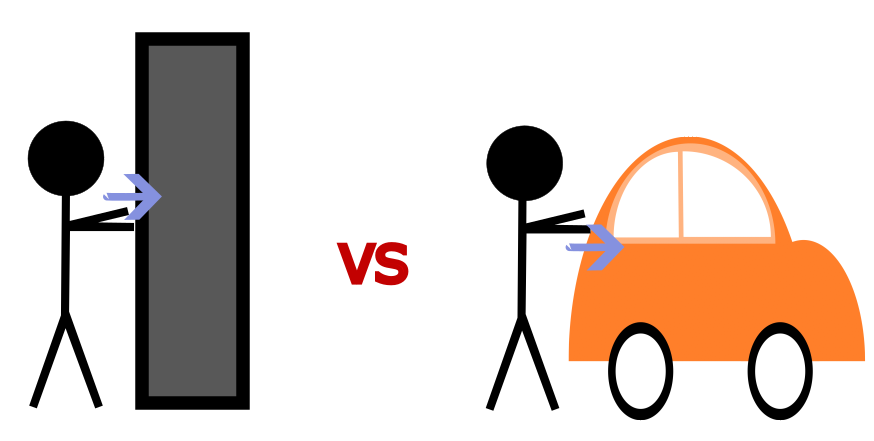
\includegraphics[width=0.8\textwidth]{Work_vs.png}

For example, if you push a car uphill with a force of 10 newtons for 12
meters, you have done 120 joules of work.\index{work}
% ADD: We can represent this with the equations, Work Energy Therom

Work is how energy is transferred from one thing to another. When you
push the car, you also burn sugars(energy of the body) in your blood. That energy is then
transferred to the car: after it has been pushed uphill.

Thus, we measure the energy something consumes or generates in 
units of work: joules, kilowatt-hours, horsepower-hours, foot-pounds,
BTUs( British Thermal Unit), and calories.

Let's go over a few different forms that energy can take.
% KA: https://www.khanacademy.org/science/ms-physics/x1baed5db7c1bb50b:energy/x1baed5db7c1bb50b:changes-in-energy/a/changes-in-energy
\section{Heat}\index{heat}

When you heat something, you are transferring energy to it. The BTU
 is a common unit for heat: One BTU is the
amount of heat required to raise the temperature of one pound of water,
by one degree. One BTU is about 1,055 joules. In fact, when you buy and sell
natural gas as fuel, it is priced by the BTU.\index{heat} \index{BTU}

\section{Electricity}\index{electricity}

Electricity is the movement of electrons. When you push electrons
through a space that resists their passage (like a light bulb),
energy is transferred from the power source ( a battery)
 into the source of the resistance.

Let's say your lightbulb consumes 60 watts of electricity, and you leave it on for 24 hours.
We would say that you have consumed 1.44 kilowatt hours or 3,600,000 joules.

% KA: https://www.khanacademy.org/science/in-in-class10th-physics/in-in-electricity/in-in-electric-current-circuit/v/intro-to-charge

\section{Chemical Energy}\index{chemical energy}

As mentioned early, some chemical reactions consume energy and some
produce energy. Thus, energy can be stored in the structure of a
molecule. When a plant uses photosynthesis to rearrange water and
carbon dioxide into a sugar molecule, it converts the energy in
the sunlight( solar energy) into chemical energy. Remember photosythesis is a process that releases energy.
Therefore, the sugar molecule has more chemical energy than the carbon dioxide and water molecules that were
used in its creation.
% ADD: photosythesis equation 
% KA: https://www.khanacademy.org/science/ap-biology/cellular-energetics/photosynthesis/a/intro-to-photosynthesis

In our diet, we measure this energy in \textit{kilocalories}. A
calorie is the energy necessary to raise one gram of water one degree
Celsius: it is about 4.19 joules. This is a very small unit: an apple
has about 100,000 calories( 100 kilocalories), so people working with food started
measuring everything in kilocalories.\index{calories}
% ADD: Conversion chapter should come before this chapter

Here is where things get confusing: People who work with food got tired of
saying ``kilocalories'', so they just started using ``Calorie'' to
mean 1,000 calories.  This has created terrible confusion over the
years. So if the C is capitalized, ``Calorie'' probably means kilocalorie.

\section{Kinetic Energy}\index{kinetic energy}

A mass in motion has energy. For example, if you are in a moving car
and you slam on the breaks, the energy from the motion of the
car will be converted into heat in the breaks and under the tires.

How much energy does the car have?
% ADD: section specifically about KE AND U, use roller coaster diagram

\begin{mdframed}[style=important, frametitle={Formula for Kinetic Energy}]

$$E = \frac{1}{2} m v^2$$

where $E$ is the energy in joules, $m$ is the mass in kilograms, and
$v$ is the speed in meters per second.

\end{mdframed}

\section{Gravitational Potential Energy}\index{potential energy!gravitational}
% KA: https://youtu.be/oGzwVYPxKjg

When you lift something heavy onto a shelf, you are giving it
\textit{potential energy}. The amount of energy that you transferred
to it is proportional to its weight and the height that you lifted it.

On the surface of the earth, gravity will accelerate a heavy object downward at
a rate of $9.8 m/s^2$.

\begin{mdframed}[style=important, frametitle={Formula for Gravitational Potential Energy}]
On earth, then, gravitational potential energy is given by

$$E = (9.8)mh$$


where $E$ is the energy in joules, $m$ is the mass of the object you
lifted, and $h$ is the height that you lifted it.

\end{mdframed}


There are other kinds of potential energy. For example, when you draw
a bow, you have given that bow potential energy. When you release it,
the potential energy is transferred to the arrow, which expresses it
as kinetic energy.
% ADD: section about KE and U

\section{Conservation of Energy}

The first law of thermodynamics says ``Energy is neither created nor
destroyed.''\index{energy!conservation of}

Energy can change forms: Your cells consume chemical energy to give
gravitational potential energy to a car you push up a hill. However, the total amount of
energy in a closed system stays constant.
% ADD: Create Systems chapter before introducing concept here

\begin{Exercise}[title={The Energy of Falling}, label=energy_falling]
  
A 5 kg cannonball falls off the top of a 3 meter ladder. Just before
it hits the floor, all of its gravitational potential energy has been
converted into kinetic energy.  How fast is the cannonball going when
it hits the floor?

\end{Exercise}
\begin{Answer}[ref=energy_falling]

  At the top of the ladder, the cannonball has $(9.8)(5)(3) = 147$ joules of potential energy.

  At the bottom, the kinetic energy $\frac{1}{2}(5)v^2$ must be equal
  to 147 joules. So $v^2 = \frac{294}{5}$.  Thus it is going about
  $7.7$ meters per second.

  (Yes, a tiny amount of energy is lost to air resistance. For a dense
  object moving at these relatively slow speeds, this energy is
  neglible.)
  
\end{Answer}


\section{Efficiency}
% KA: https://www.khanacademy.org/science/ap-biology/cellular-energetics/cellular-energy/a/the-laws-of-thermodynamics

Although energy is always conserved as it moves through different
forms, scientists aren't always that good at controlling it.\index{efficiency}

For example, a car engine consumes the chemical energy in gasoline. Only
about 20\% of the energy consumed is used to turn the wheels.  Most of
the energy is actually lost as heat. If you run a car for a while, the engine
gets very hot and the exhaust going out the tailpipe turns hot.

A human is about 25\% efficient. Most of the loss is in the heat produced
during the chemical reactions that turns food into motion.
% ADD: Cellular Respiration
 
In general, if you are trying to increase efficiency in any system,
the solution is usually easy to identify because heat is produced. Reduce heat, Increase efficiency.

Light bulbs are an interesting case. To get the light of a 60 watt
incandescent bulb, you can use an 8 watt LED or a 16 watt fluorescent
light. Thus, we say that the LED light is much more efficient: If you
run both, the incandescent bulb will consume 1.44 kilowatt-hours. The
LED will consume only 0.192 kilowatt-hours.

Besides light, the incandescent bulb is producing a lot of heat. If it
is inside your house, what happens to the heat? It warms your house.

In the winter, when you want light and heat, the incandescent bulb is
100\% efficient!

In the summer, if you are running the air conditioner, the
incandescent bulb is worse than just ``inefficient at making light'' --
it is actually counteracting the air conditioner! 

\section{Cognitive bias: Self-Serving Bias}

\newterm{Self-serving bias} is when you blame the situation for your
failures, but attribute your successes to your strengths.

For example, when asked ``Why did you lose the match?'' you are likely
to answer ``The referee wasn't fair.''  When you are asked ``Why did
you win the match?'' you are likely to answer ``Because I have been
training for weeks, and I was very focused.''

This bias tends to make us feel better about ourselves, but it makes it
difficult for us to be objective about our strengths and weaknesses.

